\chapter{Experimentos y Resultados}
\todo{escribir intro de capitulo}

\section{Colecciones}


Se seleccionan colecciones de datos multi-etiquetas del mundo real que han sido
aplicados previamente en la literatura para evaluar la capacidad predictiva de
los modelos de clasificación \cite{osojnik_multi-label_2017, read_scalable_2012,
	buyukcakir_novel_2018}. La tabla \ref{tab:datasets} enumera sus características
principales, incluyendo métricas que describen su grado de multi-etiquetado (ver
sección \ref{mll_def_formal}). Una descripción detallada de cada una se lista a
continuación:

\begin{description}

	\item{20ng} \footnote{\url{https://www.uco.es/kdis/mllresources/}}: Es una
	      colección que consta de casi 20 mil publicaciones provenientes de grupos de
	      noticias y que abordan 20 tópicos diferentes \cite{lang_newsweeder_1995}.
	      La colección es de texto y fue preprocesada para formar 1006 atributos
	      numéricos.

	\item{Enron}
	      \footnote{\url{http://sourceforge.net/projects/mulan/files/datasets/enron.rar}}:
	      Es una colección de correos electrónicos seleccionados de entre los 500 mil
	      generados por empleados de la compañía eléctrica \textit{Enron} y filtrados
	      durante una investigación por corrupción \cite{hutchison_enron_2004}. Su
	      tamaño, que no supera los 2000 elementos, no es lo suficientemente grande
	      para ser considerado un flujo continuo voluminoso, pero sí cuenta con otras
	      propiedades como la inclusión de fechas y una evolución de los datos en el
	      tiempo \cite{read_scalable_2012}. Las etiquetas se dividen en cuatro
	      grupos, según su género (acuerdos laborales, correos meramente personales,
	      etc); según la información que incluyen, esto es, si el correo contiene
	      enlaces externos, adjuntos, reenvíos, etc; según el tono emocional que
	      reflejan y según el tópico principal que abordan.

	\item{Mediamill}
	      \footnote{\url{https://sourceforge.net/projects/mulan/files/datasets/mediamill.rar}}:
	      Es una colección generada a partir de 80 horas de video provenientes de
	      transmisiones de noticias durante noviembre de 2004
	      \cite{snoek_challenge_2006}. Se seleccionaron más de 43 mil ejemplos y fue
	      manualmente etiquetada con 101 conceptos, que pueden visualizarse en la
	      figura \ref{fig:mediamill}.

\end{description}

\begin{table}[h]
	\centering
	\label{tab:datasets}
	\begin{tabular}{llrrrrr}
		\toprule
		Nombre    & Dominio & N     & A    & L   & LC    & LD    \\
		\midrule
		20ng      & Texto   & 19300 & 1006 & 20  & 1,029 & 0,051 \\
		Enron     & Texto   & 1702  & 1001 & 53  & 3,378 & 0,064 \\
		Mediamill & Video   & 43907 & 120  & 101 & 4,376 & 0,043 \\
		\bottomrule
	\end{tabular}
	\caption{Colecciones multi-etiquetas y sus características. N: número de
		instancias; A: número de atributos; L: número de etiquetas; LC: cardinalidad
		de etiquetas; LD: densidad de etiquetas.}
\end{table}

\begin{figure}
	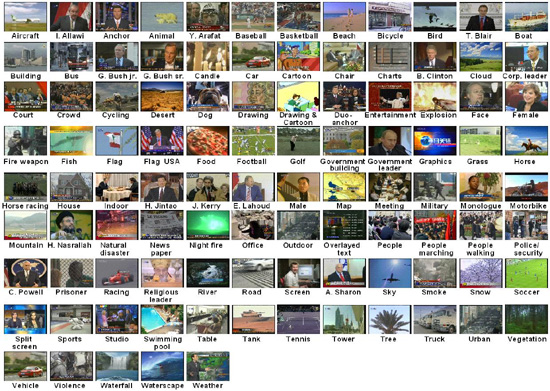
\includegraphics[width=.9\linewidth]{figures/mediamill.jpg}
	\centering
	\caption{Los 101 conceptos semánticos asociados a la colección
		Mediamill.}
	\label{fig:mediamill}
\end{figure}

Estas son sólo tres de las colecciones usualmente abordadas en la literatura y
se han seleccionado con el objetivo de diversificar el análisis. Enron es una
colección de pocas instancias pero muchas etiquetas, 20ng a la inversa, cuenta
con pocas etiquetas pero muchas instancias; y Mediamill, finalmente, es la
colección con más instancias que hay disponible y cuenta también con un número
relativamente alto de etiquetas.

Durante la ejecución de experimentos, cada colección será convertida a un flujo
sintético. Además, se generará una versión sintética de cada una, siguiendo la
técnica descripta en la sección \ref{generacion_flujos_sinteticos}.

\section{Software}

A continuación se describen las herramientas de software que fueron utilizadas
para la implementación y ejecución de los experimentos.

\begin{description}

	\item[scikit-multiflow]\footnote{\url{https://scikit-multiflow.github.io/}} Es
	      una librería disponible para el lenguaje de programación Python que provee
	      un \textit{framework} para implementar y comparar algoritmos de aprendizaje
	      automático en ambientes de flujos continuos de datos. Incluye pero no se
	      limita a problemas de clasificación multi-etiquetas
	      \cite{montiel_scikit-multiflow_2018}.

	\item[\acrshort{moa}]\footnote{\url{https://moa.cms.waikato.ac.nz/}}
	      \acrfull{moa} es un \textit{framework} para realizar minería de datos sobre
	      flujos continuos de datos, implementada en Java y de código libre.  Incluye
	      algoritmos de evaluación y de aprendizaje automático como clasificadores,
	      regresores, o de \textit{clustering}, pudiendo ser aplicados a problemas de
	      clasificación de etiqueta única o multi-etiquetas.  También incluye
	      herramientas para generar datos sintéticos. Tanto \acrshort{moa} como
	      scikit-multiflow facilitan la reiteración de experimentos con distintas
	      configuraciones, así como la comparación de resultados y la extensión de
	      funcionalidad \cite{bifet_moa_2010}.

	\item[scikit-learn]\footnote{\url{http://scikit-learn.org/stable/index.html}}
	      Es una librería del lenguaje de programación Python que brinda
	      herramientas para realizar evaluación, visualización y análisis de
	      resultados \cite{pedregosa_scikit-learn_2018}.

	\item[Mulan]\footnote{\url{http://mulan.sourceforge.net/index.html}} Es una
	      librería del lenguaje Java especializada en aprendizaje por
	      multi-etiquetas. Mulan incluye una variedad de colecciones de datos
	      multi-etiquetas que han sido la fuente de otros trabajos de la literatura
	      \cite{tsoumakas_mulan_2011}.

\end{description} \todo{nombres de herramientas van en cursiva?}

La herramienta \acrshort{moa} es usada para generar los flujos sintéticos y
provee del marco de trabajo en el cual se implementó el algoritmo de generación
descripto en \ref{generacion_flujos_sinteticos}. Los algoritmos de clasificación
fueron implementados en Python y están disponibles bajo la librería
\textit{scikit-multiflow}. La solución de ensamble \acrshort{efmp} también fue
implementada en esta librería. \textit{scikit-learn}, por su parte, provee la
implementación de las métricas basadas en etiquetas, y las colecciones de datos
fueron extraídas de mulan.

\section{Hardware}

Se ha recibido apoyo del \acrfull{cidetic}, el cual ha proveído de equipos de
altas prestaciones que han proporcionado la capacidad de cómputo necesaria para
llevar a cabo este proyecto. El equipamiento facilitado cuenta con dos nodos de
12 núcleos cada uno, el CPU es un Intel Xeon X5675 de 3.07 GHz de velocidad de
procesamiento, 12 Mb de memoria caché y 6 núcleos. El espacio de almacenamiento
disponible es de 1 Tb y la memoria RAM es de 142 Gb. \todo{Chequear estos datos}

El Sistema Operativo instalado es Ubuntu 18.04 LTS y cuenta con la versión 3.6.9
de Python, el instalador de paquetes Pip en su versión 20.3.3 y Java 1.8.

\section{Algoritmos}
\label{experimentos_algoritmos}

Se realizan los experimentos usando algoritmos multi-etiquetas disponibles en la
librería scikit-multiflow junto con la implementaciones de ensamble presentada
en este trabajo, \acrfull{efmp} y su variación \acrshort{efmp2}. Entre los
algoritmos del tipo de transformación del problema se seleccionan los de
\acrfull{br}, \acrfull{cc} y \acrfull{mlht}. Tanto \acrshort{br} como
\acrshort{cc} usan \textit{naive} bayes como modelo de clasificación base y
\acrshort{mlht} es ejecutado en su versión basada en \acrfull{lp}, siguiendo los
procedimientos de \citeauthor{read_scalable_2012} \cite{read_scalable_2012}.

En lo que respecta a soluciones de ensamble, los modelos de \acrshort{efmp}
contarán ambos con tres clasificadores base, siendo estos los mencionados en el
párrafo anterior, es decir, \acrshort{cc}, \acrshort{br} y \acrshort{mlht}. La
comparación se hará contra el algoritmo \acrfull{dwm}, tal como ha sido definido
por sus autores \cite{kolter_dynamic_2007} pero adaptado a ambientes de
multi-etiquetas (ver sección \ref{tecnica_algoritmo_ensamble}), y se suman al
análisis los algoritmos de \acrfull{ebr} y \acrfull{ecc}, tal como fueron
definidos por \citeauthor{oza_online_2005} \cite{oza_online_2005} y también han
sido extendidos para soportar problemas de \acrshort{mll}
\cite{read_classifier_2011}. Los tres algoritmos de ensamble extraídos de la
literatura son configurados con diez clasificadores base de \textit{naive}
bayes, para imitar los experimentos conducidos por otros autores de la
literatura \cite{osojnik_multi-label_2017, read_scalable_2012,
	buyukcakir_novel_2018}.

La tabla \ref{tab:algoritmos} es un resumen de los algoritmos seleccionados
junto con los clasificadores base configurados, la referencia bibliográfica y la
clave que será usada en las tablas de resultados.

\begin{table}[h]
	\centering
	\label{tab:algoritmos}
	\begin{adjustbox}{max width=\textwidth}
		\begin{tabular}{lllll}
			\toprule
			Clave                                          & Algoritmo                             & Clasificadores base  & Referencia & \\
			\midrule
			\acrshort{br}                                  & \acrlong{br}                          & \textit{naive} bayes
			                                               & \textcite{tsoumakas_multi-label_2007} &                                     \\
			\acrshort{cc}                                  & \acrlong{cc}                          & \textit{naive} bayes &
			\textcite{read_classifier_2011}                &                                                                             \\
			\acrshort{mlht}                                & \acrlong{mlht}                        & \acrfull{ht}         &
			\textcite{read_scalable_2012}                  &                                                                             \\
			\acrshort{efmp}                                & \acrlong{efmp}                        &
			\acrshort{br}, \acrshort{cc} y \acrshort{mlht} &
			Sección \ref{tecnica_algoritmo_ensamble}       &                                                                             \\
			\acrshort{efmp2}                               & \acrlong{efmp2}                       &
			\acrshort{br}, \acrshort{cc} y \acrshort{mlht} &
			Sección \ref{tecnica_algoritmo_ensamble}       &                                                                             \\
			\acrshort{dwm}                                 & \acrlong{dwm}                         &
			\textit{naive} bayes (10 copias)               &
			\textcite{kolter_dynamic_2007}                 &                                                                             \\
			\acrshort{ebr}                                 & \acrlong{ebr}
			                                               & \textit{naive} bayes (10
			copias)                                        &
			\textcite{read_classifier_2011}                &                                                                             \\
			\acrshort{ecc}                                 & \acrlong{ecc}
			                                               & \textit{naive} bayes (10
			copias)                                        &
			\textcite{read_classifier_2011}                &                                                                             \\
			\bottomrule
		\end{tabular}
	\end{adjustbox}
	\caption{Métodos de clasificación multi-etiquetas seleccionados para ambientes
		de flujos continuos de datos.}
\end{table}

\section{Métricas de Evaluación}

En la evaluación de algoritmos de clasificación se usan el conjunto de métricas
que han sido utilizadas en otros trabajos de la literatura, tanto en escenarios
de flujos \cite{sousa_multi-label_2018, zheng_survey_2020,
	osojnik_multi-label_2017} como en \textit{batch} \cite{madjarov_extensive_2012,
	zhang_multi-label_2010, gibaja_tutorial_2015} y fueron descriptas en la
sección \ref{mll_evaluacion}. Estas son:

\begin{description}

	\item[Métricas Basadas en Ejemplos]: \textit{Hamming score}, exactitud del
	      subconjunto, exactitud (ejemplos), precisión (ejemplos), exhaustividad
	      (ejemplos) y medida-f1 (ejemplos).

	\item[Métricas Basadas en Etiquetas]: Micro-exactitud, micro-precisión,
	      micro-exhaustividad, micro-f1, macro-exactitud, macro-precisión,
	      macro-exhaustividad y macro-f1.

	\item[Métricas de Eficiencia]: Velocidad y consumo de memoria.

\end{description}

La medición de velocidad comienza en el momento que inicia la predicción y
entrenamiento del modelo por primera vez y finaliza cuando el clasificador
termina de procesar la última instancia de la colección. Por lo tanto, quedan
afuera las etapas de evaluación, carga de la colección en memoria, generación
del flujo y configuración del entrenamiento. El consumo de memoria también es
monitoreado durante la ejecución del entrenamiento y predicción y toma en cuenta
la estructura completa del modelo y todos sus componentes, incluyendo pesos e
hiper-parámetros propios y de sus clasificadores base.

Los flujos sintéticos son analizados teniendo en cuenta los fenómenos propios de
colecciones del mundo real. A ese fin se estudia el sesgo de etiquetas, la
relación entre etiquetas, la distribución de etiquetas y el espacio de atributos
(ver sección \ref{mll_fenomenos}). \todo{es probable que este análisis se separe
	en una sección aparte y se aborde con mayor profundidad}

\section{Configuración Experimental}

En lo que respecta a modelos de aprendizaje automático, los experimentos fueron
desarrollados en el lenguaje Python usando la librería
\textit{scikit-multiflow}. Los algoritmos de transformación del problema se
aplican tal como han sido implementados en la librería con la salvedad del
\acrshort{mlht}, al que debió introducirle una modificación para manipular la
predicción, se usaba un arreglo disperso para representar las etiquetas
activadas, lo cual producía un desbordamiento de memoria en el entrenamiento de
colecciones grandes como la de mediamill. Se lo suplantó por una estructura de
representación densa. En cuanto a los modelos de ensambles, se adaptaron las
implementaciones existentes de \acrshort{ebr}, \acrshort{ecc} y \acrshort{dwm}
para soportar múltiples etiquetas y para ello se debió modificar la etapa de
combinación de votos para hacer frente a la nueva dimensionalidad de los datos.
Por lo demás, la configuración de los algoritmos es la definida en la sección
\ref{experimentos_algoritmos}.

Para la etapa de evaluación se aplica la técnica de evaluación secuencial
predictiva (\textit{prequential}) con ventanas deslizantes, tal como se
recomienda para ambientes de flujos continuos \cite{gama_evaluating_2013}. Ante
cada ejemplo o ventana de ejemplos arribada el modelo primero realiza la
predicción y luego el entrenamiento. Finalmente las métricas de evaluación son
calculadas una vez procesados todos los ejemplos de la colección y a partir de
todas las predicciones producidas.  Notar que a partir de esta técnica el modelo
predice y entrena todas las instancias, y no solo un subconjunto de ellas como
sucede con la estrategia de \textit{holdout}. La ventana deslizante se configura
en $w = \frac{N}{20}$, es decir, se divide el número total de instancias del
flujo en 20 ventanas, siguiendo las directivas de \textcite{read_scalable_2012}.
Los resultados de la evaluación son agrupados según los tipos de métrica usados,
para facilitar el análisis.

Por otro lado, los flujo de datos sintéticos fueron generados a partir de las
colecciones 20ng, enron y mediamill, y cada una cuenta con cien mil instancias.
Sus atributos se generan usando el algoritmo \acrfull{rbf} (ver sección
\ref{stream_syn}).

\section{Resultados}
